\documentclass{article}
\usepackage{fasy-hw}

\author{Joshua Harthan}
\problem{1}
\begin{document}
Use induction to prove that a tree always has one more vertex than edges.
\item[] 
    \begin{proof}
        \caption{}
         First, let's represent the number of vertices within a tree to be $v$ while the number of edges within a tree is $e$, where both $v$ and $e$ are integers. Then, let's let P($v$) be: Any tree with $v$ vertices has $v - 1$ edges. First, we must show that P(1) is true. Let $T$ be any tree with one vertex. $T$ has zero edges, and therefore we are given the equation 0 = 1 - 1 making P(1) true. 
        \item[] From here, we must show that for all integers $k \geq 1$, if P($k$) is true, then P($k+1$) is also true. To do this, let's suppose that any tree with $k$ vertices has $k - 1$ edges, and show that for any tree $T$ with $k + 1$ vertices has ($k + 1) - 1 = k$ edges. If we let $T$ be a tree with $k + 1$ vertices, giving us $(k + 1) \geq 2$, which tells us that $T$ has more than one vertex. Since $T$ has more than one vertex, $T$ has vertex of degree 1, let's call it $v$. Since $T$ is a tree, there must be an edge $e$ connecting $v$ to the rest of $T$. If we define a different tree within $T$ called $A$, where the number of vertices in $A$ is the number of vertices within $T - v$, and the number edges in $A$ is the number of edges within $T - e$, we can say that the number of vertices within $A$ is $(k + 1) - 1 = k$. Therefore the number of edges of $A$ are $k$ (the number of vertices within $A$) subtracted from 1, or just $k - 1$. Therefore, by induction, a tree always has one more vertex than edges.
        \end{proof}


\problem{2}
\collab{none}
\clearpage
\header
Use Master's theorem to solve the following recurrence relations. If you use cases one or three, be sure to state what $\epsilon$ should be.
\item[]2.1 $T(n) = 9 T(n/3) + n$
\item[]2.2 $T(n) = T(n/2) + 1$
\item[]2.1 From Master's Theorem, we get values $a$ = 9, $b$ = 3, and $f(n) = n$. If we let $\epsilon$ = 1, then $n^{log_{3}9 - 1}$ gives us $f(n) = $ O$(n^{2-1}) = $ O($n$). Therefore, from Case 1 of Master's Theorem, $T(n)$ is $\Theta(n^{log_{3}9}) = \Theta(n^{2})$.
\item[]2.2 From Master's Theorem, we get values $a$ = 1, $b$ = 2, and $f(n) = 1$. From this, we get $f(n) = \Theta(n^{log_{2}1}) = \Theta(n^{0}) = \Theta(1)$. Therefore, from Case 2 of Master's Theorem, $T(n)$ is $\Theta(n^{0}logn)$ = $\Theta(logn)$. 

\problem{3}
\collab{none}
\clearpage
\header
The following is an encrypted message: DUR OR MNSG.
\item[](a) What is the decoded message?
\item[](b) How did you determine what the message was? Explain what you tried, both the successful, and the unsuccessful attempts, if applicable. If known, explain what the encryption key is.
\item[](a) The decoded message is LET IT SNOW.
\item[](b) Using an affine cipher, and the decryption function: $D(x) = a^{-1}(x-b)$ mod $m$, where $a$ and $b$ are the encryption keys, $x$ is the number of the letter in the alphabet subtracted from one, and $m$ is the size of the alphabet, i.e. 26. To calculate $a^{-1},$ we can use the equation $1 = aa^{-1}$ mod $m$, to find $a^{-1}$ = 21. We can represent DUR OR MNSG as 3 20 17 14 17 12 13 18 6. Using the equation, $D(x) = 21(y)$ mod 26 for each value of y, we get 11 4 19 8 19 18 13 14 22. Taking theses values back to their alphabetical values gives us LET IT SNOW. The encryption keys are $a$ = 5 and $b$ = 0.


\problem{4}
\collab{none}
\clearpage
\header
9.3 Question 30
\item[]Assuming that all years have 365 days and all birthdays occur with equal probability, how large must $n$ be so that in any randomly chosen group of $n$ people, the probability that two or more have the same birthday is at least 1/2?
\item[]To solve this, we can say that the probability that two people share the same birthday is $P(N)$, and the probability of two people not sharing the same birthday can be represented by $P(N) = 1 - P(N')$. $P(N') = \frac{365!}{365^{n}(365 - n)!}$, and we want $P(N')$ to be 50\%. From this equation, $P(N') = \frac{365!}{365^{n}(365 - n)!} = .5$ and solving for $n$, we get $n$ to be around 23. Therefore, the least amount of people for the probability of two people to share a birthday to be 50\% is 23.


\problem{5}
\collab{none}
\clearpage
\header
What is the dual graph of Example 1 (page 9 of Wilson)?
\begin{figure}[h!]
  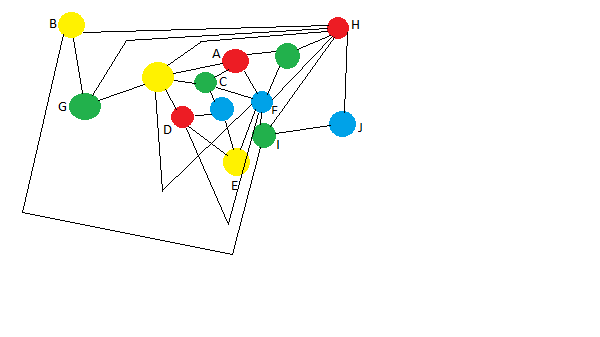
\includegraphics[width=\linewidth]{Untitled.png}
  \caption{Dual Graph of Example 1}
  \label{fig:map1}
\end{figure}


\problem{6}
\collab{none}
\clearpage
\header
Grace Hopper was an American computer scientist most known for her work on programming on the Harvard Mark 1 computer, her work on inventing one of the first compilers, and her popularization of high-level programming languages with her development of COBOL. COBOL, still used today in business and administrative systems for companies, is an English-like programming language that was meant to be easier to use and to implement. Without computer scientists like Grace Hopper, who pioneered certain elements within computer science, we wouldn't have many elements within today's programming languages.

\item[]\url{https://en.wikipedia.org/wiki/Grace_Hopper}
\item[]\url{https://en.wikipedia.org/wiki/COBOL}
\end{document}